\documentclass[handout]{beamer}

\usepackage{amsmath}
\usepackage{float}
\usepackage{graphicx}
\usepackage{url}
\usepackage{ulem}

\usepackage{../recdefs}

\usetheme{CambridgeUS}

\title{CS100 Recitation 1}
\author{GKxx}
\date{Februrary 21, 2022}

\begin{document}

\begin{frame}
    \maketitle
\end{frame}

\AtBeginSubsection[]{
    \begin{frame}{Contents}
        \tableofcontents[currentsection, currentsubsection]
    \end{frame}
}

\section{C/C++ Environment Setting up}

\subsection{Basic Knowledge}

\begin{frame}{Editors, Compilers and IDEs}
    \begin{itemize}
        \item A \blue{compiler} translates the program written in a high-level language so that the computer can run it.
        \begin{itemize}
            \item \texttt{GCC}, \texttt{Clang}, \texttt{Visual C++} compiler, \dots
        \end{itemize}
        \pause
        \item An \blue{editor} is something where you can edit text.
        \begin{itemize}
            \item \texttt{Notepad}, \texttt{Word}, and even your phone memo.
            \pause
            \item But we need a \blue{code editor} which provides more help for coding.
            \item \texttt{Visual Studio Code}, \texttt{Vim}, \texttt{Sublime Text}, \texttt{Notepad++}, \dots
        \end{itemize}
        \pause
        \item IDE: \textbf{I}ntegrated \textbf{D}evelopment \textbf{E}nvironment,
        \begin{itemize}
            \item \(=\) editor \(+\) compilers \(+\) debuggers \(+\cdots\).
            \item \texttt{Visual Studio}, \texttt{Qt}, \texttt{CLion}, \texttt{Dev-C++}, \dots
        \end{itemize}
    \end{itemize}
\end{frame}

\subsection{Installation of Compiler}

\begin{frame}{GCC and MinGW}
    \begin{itemize}
        \item \blue{GCC} is the \textbf{G}NU \textbf{C}ompiler \textbf{C}ollection, an optimizing compiler produced by the \blue{GNU Project} supporting various \blue{programming languages}, \blue{hardware architectures} and \blue{operating systems}.
        \item \blue{MinGW} is short for \textbf{Min}imalist \textbf{G}NU for \textbf{W}indows.
        \pause
        \item For Linux, install GCC directly is ok.
        \item For Windows, you may need MinGW (or, probably MinGW-w64).
    \end{itemize}
\end{frame}

\begin{frame}{MinGW}
    \begin{itemize}
        \item Download the package provided in the Resources page.
        \item Unzip it and place the \texttt{mingw64} folder in the \texttt{C} drive.
        \begin{figure}[h]
            \centering
            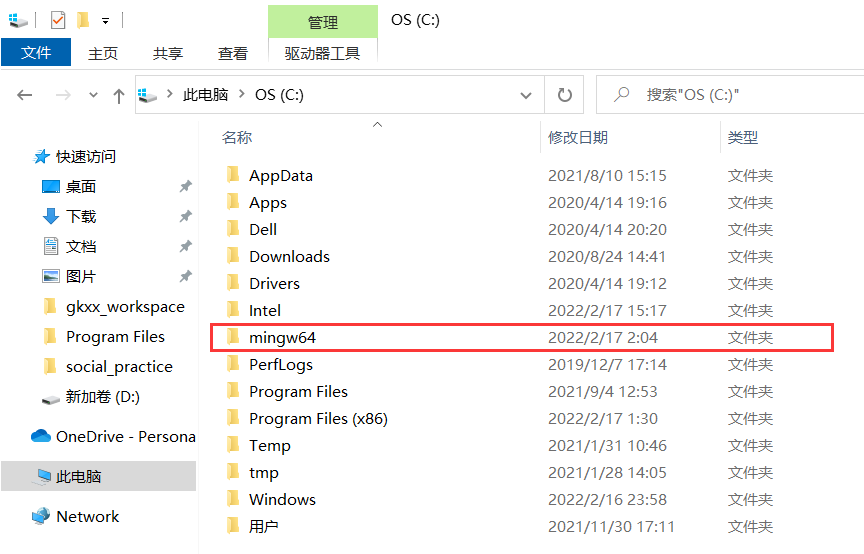
\includegraphics[width=0.8\textwidth]{img/mingw_in_c.png}
        \end{figure}
    \end{itemize}
\end{frame}

\begin{frame}{MinGW}
    \begin{itemize}
        \item Now the compiler is installed, but it could not be invoked conveniently. We need to add it to the \texttt{Path} \blue{environment variable}.
        \item Press \texttt{Win} and search `env'. Choose `Edit the system environment variables'.
        \begin{figure}[h]
            \centering
            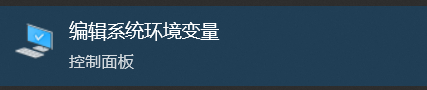
\includegraphics[width=0.5\textwidth]{img/start_env.png}
        \end{figure}
        \item Click the `Environment variables ...' button.
    \end{itemize}
\end{frame}

\begin{frame}{MinGW}
    \begin{figure}[h]
        \centering
        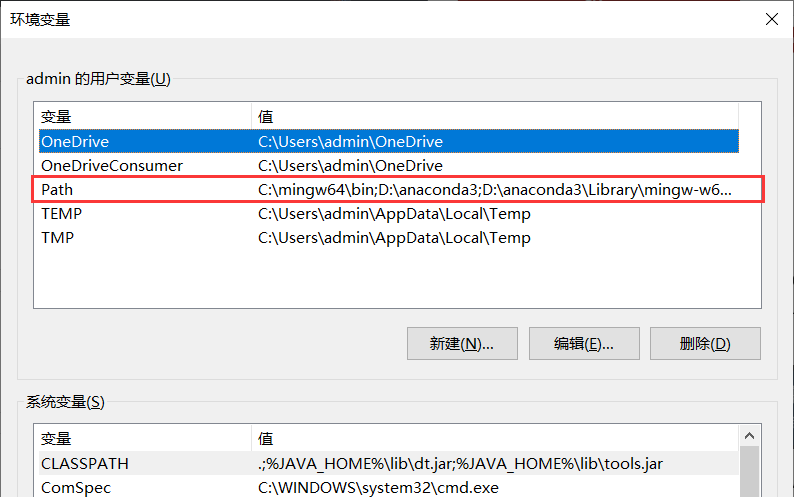
\includegraphics[width=0.8\textwidth]{img/env_var.png}
    \end{figure}
\end{frame}

\begin{frame}{MinGW}
    \begin{itemize}
        \item Add a new value `\texttt{C:\textbackslash mingw64\textbackslash bin}'.
        \begin{figure}[h]
            \centering
            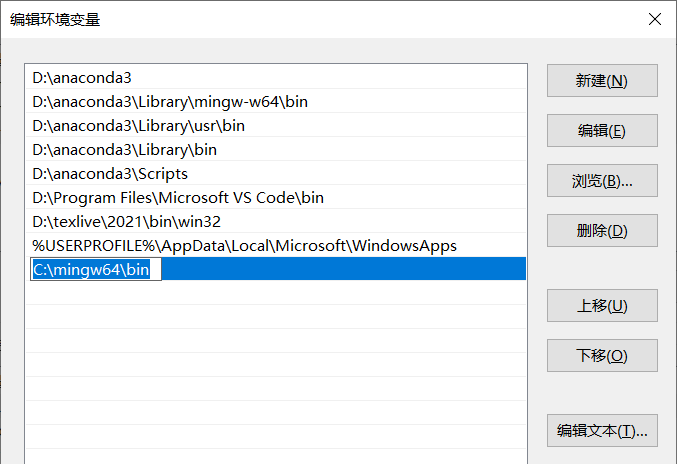
\includegraphics[width=0.8\textwidth]{img/added.png}
        \end{figure}
    \end{itemize}
\end{frame}

\begin{frame}{MinGW}
    \begin{itemize}
        \item Press \texttt{Win}\(+\)\texttt{r} to open a cmd.
        \item Type `gcc' and press \texttt{Enter}. The following shows that \texttt{gcc} is correctly invoked.
        \begin{figure}[h]
            \centering
            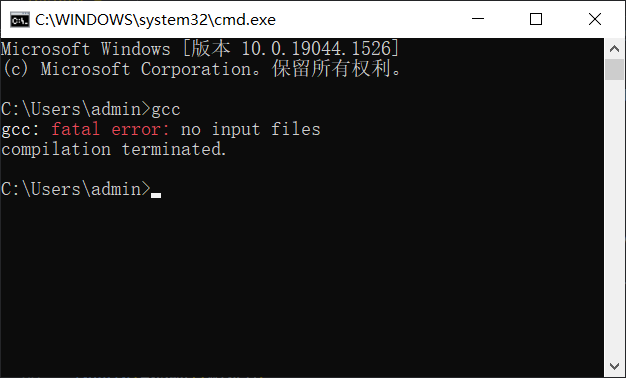
\includegraphics[width=0.8\textwidth]{img/cmd_gcc.png}
        \end{figure}
    \end{itemize}
\end{frame}

\begin{frame}{MinGW}
    You can use `\texttt{--version}' to see more information about the compilers.
    \begin{figure}[h]
        \centering
        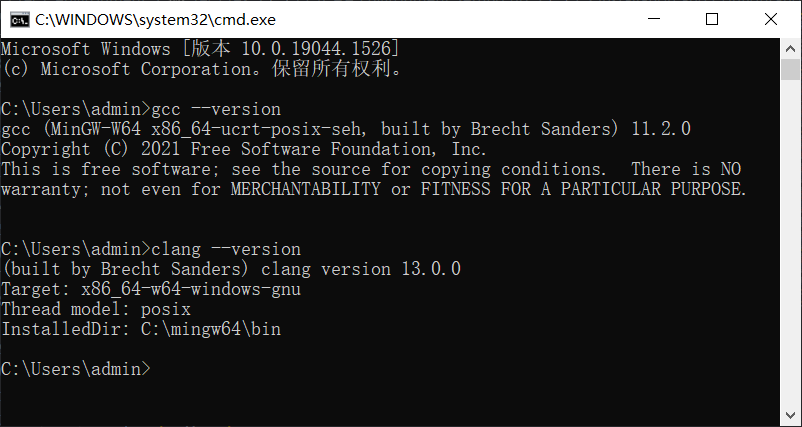
\includegraphics[width=0.8\textwidth]{img/compiler_versions.png}
    \end{figure}
\end{frame}

\begin{frame}{For Linux (Ubuntu)}
    \begin{itemize}
        \item `\texttt{sudo apt install build-essential}' gets everything done.
        \item If you want compilers of newer version:\\
        \texttt{sudo add-apt-repository ppa:ubuntu-toolchain-r/test}\\
        \texttt{sudo apt update}\\
        \texttt{sudo apt install gcc-11}\\
        \texttt{sudo apt install g++-11}
        \item `\texttt{sudo apt install clang-12}'. For the latest version \texttt{Clang-13}:\\
        \texttt{wget https://apt.llvm.org/llvm.sh}\\
        \texttt{sudo chmod a+x llvm.sh}\\
        \texttt{sudo ./llvm.sh 13}
        \item You can search for more on your own.
    \end{itemize}
\end{frame}

\begin{frame}{For Mac OS X}
    \begin{figure}[h]
        \centering
        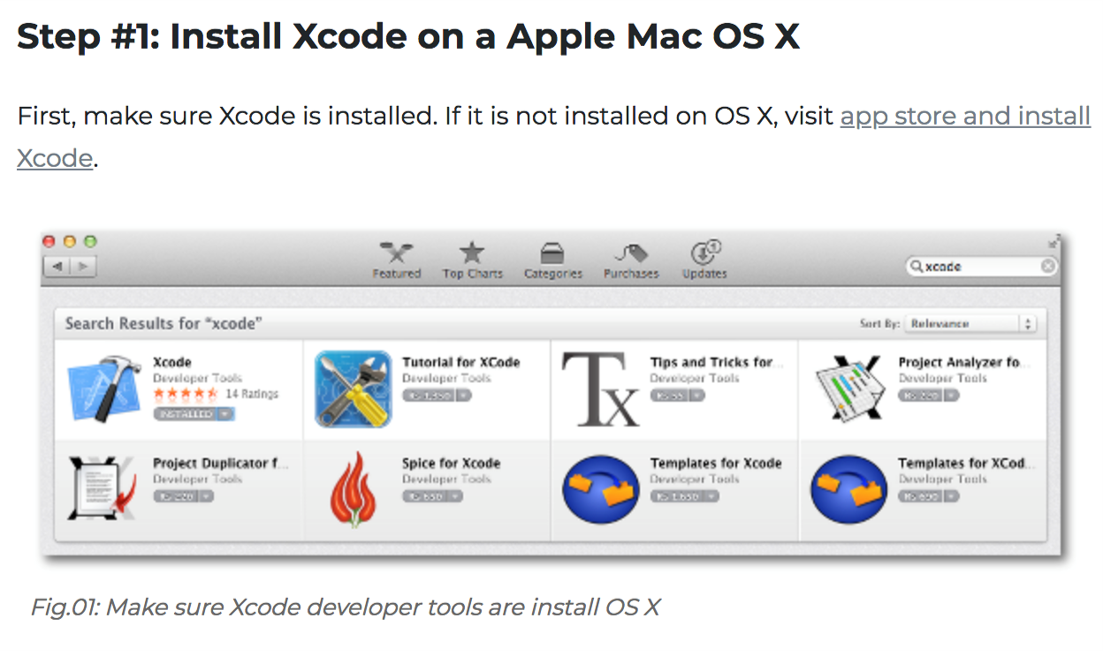
\includegraphics[width=0.9\textwidth]{img/install_xcode.png}
    \end{figure}
\end{frame}

\begin{frame}{For Mac OS X}
    \begin{figure}[h]
        \centering
        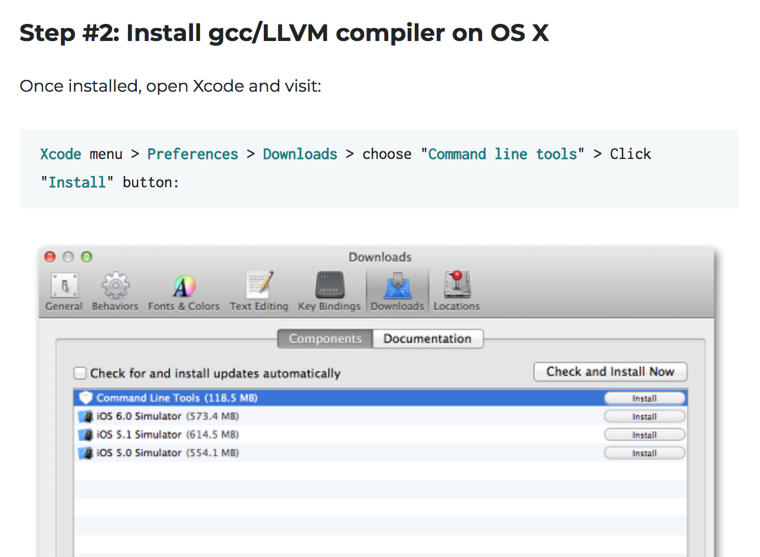
\includegraphics[width=0.8\textwidth]{img/install_cmd_tools.png}
    \end{figure}
\end{frame}

\begin{frame}{For Mac OS X}
    \begin{figure}[h]
        \centering
        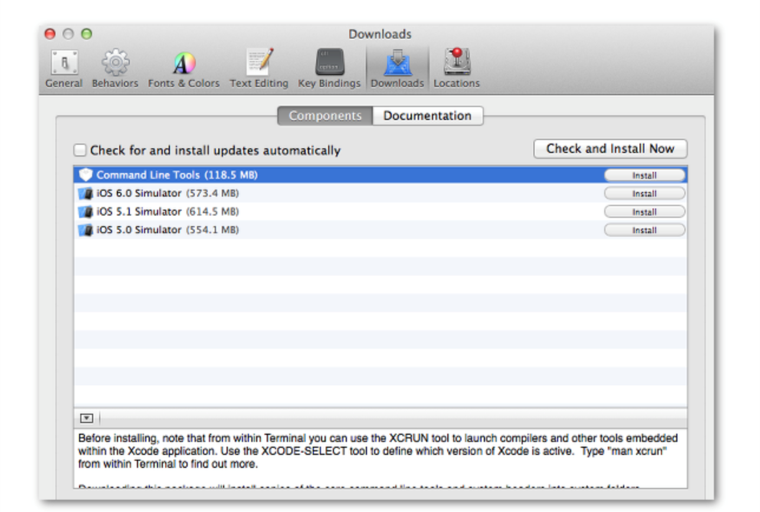
\includegraphics[width=0.9\textwidth]{img/install_cmd_tools_2.png}
    \end{figure}
\end{frame}

\begin{frame}{For Mac OS X}
    \begin{itemize}
        \item Verify that it is working: `\texttt{gcc --version}'
    \end{itemize}
    \begin{figure}[h]
        \centering
        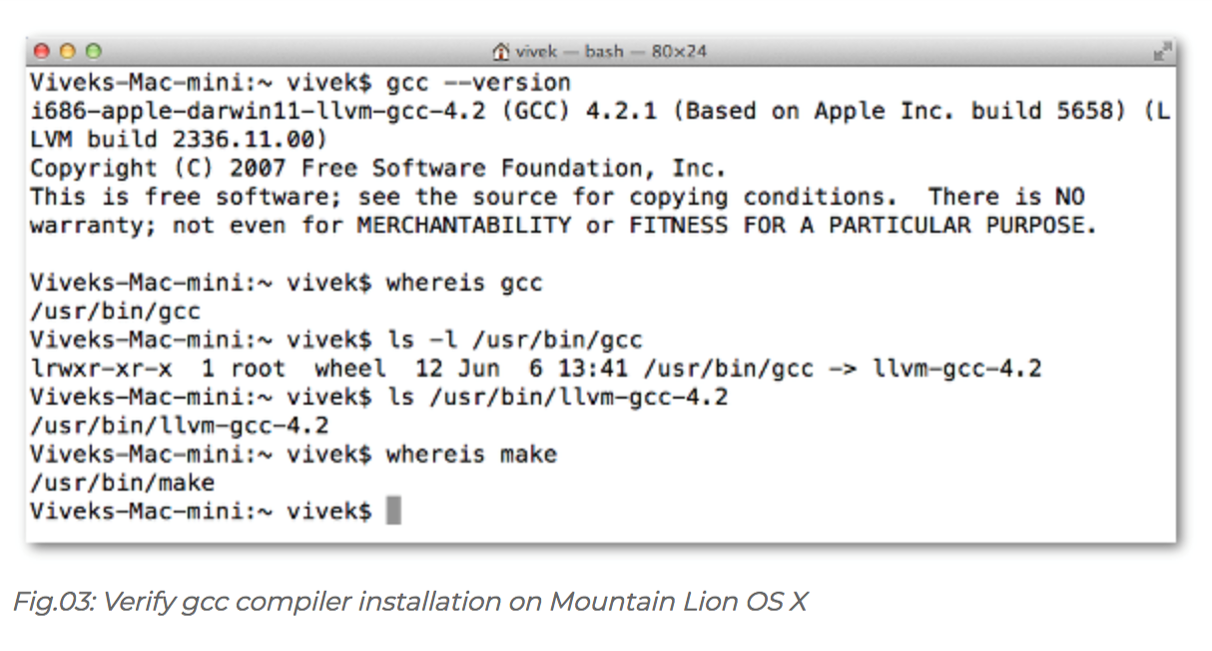
\includegraphics[width=0.9\textwidth]{img/mac_verify_gcc.png}
    \end{figure}
\end{frame}

\subsection{Installation and Configuration of VSCode}

\begin{frame}{Installation}
    \begin{itemize}
        \item Install \texttt{VSCode} from \url{code.visualstudio.com}.
        \item For Linux users, \textbf{DO NOT} install it via \texttt{snap} or you may encounter trouble.
        \pause
        \item Run the installer. It is recommended to install it in the \texttt{D} or \texttt{E} drive, e.g. \texttt{D:\textbackslash Program Files\textbackslash Microsoft VS Code\textbackslash}.
    \end{itemize}
\end{frame}

\begin{frame}{Extensions}
    Recommended extensions:
    \begin{itemize}
        \item \texttt{Code Runner}, \texttt{C/C++}, \texttt{C++ Intellisense}.
        \item \texttt{Bracket Pair Colorization Toggler}, \texttt{vscode-icons}.
        \item \texttt{One Dark Pro} and \texttt{GitHub Theme}: color themes.
        \item \sout{\texttt{GlassIt-VSC}, \texttt{Cloudmusic}, \texttt{QQ}, \texttt{Zhihu On VSCode}, \dots}
    \end{itemize}
    You may also need \texttt{Chinese (Simplified) Language Pack for Visual Studio Code}.
\end{frame}

\begin{frame}{Configuration}
    \begin{itemize}
        \item Create a folder for CS100, e.g. \texttt{D:\textbackslash CS100}. This will be viewed as a \blue{workspace}.
        \pause
        \item \texttt{VSCode} has `\(n+1\)' configurations, where \(n\) is the number of workspaces and the `\(+1\)' refers to the global (user's) one.
        \item The configuration of each workspace is done by some \texttt{json} files in a special folder \texttt{.vscode}.
        \pause
        \item Remember to always \blue{open \texttt{VSCode} first and then open the workspace}, instead of open a single file directly. Otherwise your configuration for workspace wouldn't work.
    \end{itemize}
\end{frame}

\begin{frame}{Configuration}
    Global settings:
    \begin{figure}[h]
        \centering
        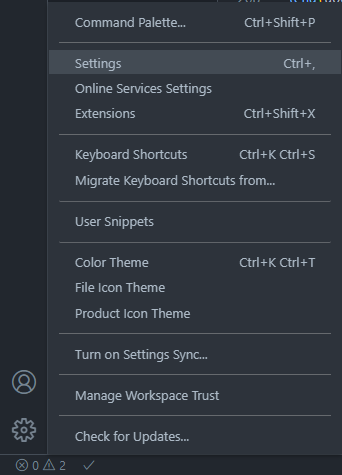
\includegraphics[height=0.75\textheight]{img/vsc_global.png}
    \end{figure}
\end{frame}

\begin{frame}{Configuration}
    Recommended global settings:
    \begin{itemize}
        \item Code-runner: Save File Before Run\quad\blue{true}
        \item Code-runner: Run In Terminal\quad\blue{true}
        \item Code-runner: Ignore Selection\quad\blue{true}
        \item Editor: Format On Save\quad\blue{true}
    \end{itemize}
\end{frame}

\begin{frame}{Configuration}
    \begin{itemize}
        \item Create a folder \texttt{D:\textbackslash CS100\textbackslash .vscode} for your workspace configurations.
        \item Create two files \texttt{settings.json} and \texttt{c\_cpp\_properties.json}. Copy the contents from \url{https://www.luogu.com.cn/paste/scc7i5yq}.
        \pause
        \item Create a hello-world program somewhere in this workspace, e.g. \texttt{D:\textbackslash CS100\textbackslash tmp\textbackslash hello.c}.
        \item There will be a `Run Code' button on the top-right corner. Or you can press \texttt{Ctrl+Alt+N} to run the code.
    \end{itemize}
\end{frame}

\begin{frame}{Configuration}
    \begin{itemize}
        \item Pressing this button, the \texttt{Code Runner} extension runs the command we wrote in \texttt{"code-runner.executorMap"} in \texttt{settings.json}.
        \item It is running in the terminal of \texttt{VSCode}, which is the same as in cmd.
        \item The \texttt{Code Runner} extension gets you free from typing the same compilation command manually over and over again. (You may have a try of typing it manually.)
        \item \blue{If the terminal in \texttt{VSCode} cannot recognize the compiler, just reboot the computer.}
    \end{itemize}
\end{frame}

\begin{frame}{Configuration}
    For the debugging part:
    \begin{itemize}
        \item Print statement debugging is effective, although \texttt{VSCode} says that it is `a thing of the past'.
        \item To use the tools for debugging in \texttt{VSCode}, press \texttt{F5}.
        \item Choose `GDB/LLDB', and then choose `gcc'. If you wish to use the LLVM debuggers, you need to install `lldb-mi' on your own.
        \item Wait a second and the default configuration files for debugging (\texttt{launch.json} and \texttt{tasks.json}) are generated automatically.
        \pause
        \item[\(\Rightarrow\)] An example: the ``A+B'' problem.
    \end{itemize}
\end{frame}

\section{Preparation}

\begin{frame}{Where Do I Learn Things?}
    \begin{itemize}
        \item More about \texttt{VSCode}, you can visit the official website \url{code.visualstudio.com}.
        \item \textbf{You should get used to reading official documentations}, not only for \texttt{VSCode}, but also for most programming languages and tools.
        \pause
        \item The official documentation for \texttt{C/C++} is not suitable for newcomers. We recommend \url{cppreference.com}.
    \end{itemize}
\end{frame}

\begin{frame}{Where Do I Learn Things?}
    Apart from the course and slides, we can learn things from:
    \begin{itemize}
        \item \url{stackoverflow.com}, mostly for bug-fixing and trouble-shooting. (Also \url{stackexchange.com})
        \item \url{cppreference.com} and \textbf{authoritative} textbooks like \textit{C++ Primer}. One may use them as a dictionary.
        \item books like \textit{Effective C++}, which helps you solve common problems and develop good coding habits.
    \end{itemize}
\end{frame}

\begin{frame}{Where Do I Learn Things?}
    The following websites do offer some help, but are not recommended:
    \begin{itemize}
        \item Wikipedia and Baidu Baike: Everyone can edit, and some contents are checked by experts.
        \item Zhihu, CSDN, Luogu, and some other blogs. Everyone can edit and no one checks.
        \item Baidu Zhidao, Baidu Jingyan, Xiao Hongshu: No experts would be willing to write things there!
    \end{itemize}
\end{frame}

\section{Foundations of C}

\subsection{Language Standards}

\begin{frame}{Language Standards}
    \begin{itemize}
        \item Standards of C: C89/90, C99, C11, C17, C23 (coming soon).
        \item Standards of C++: C++98/03, C++11, C++14, C++17, C++20, C++23 (coming soon),\dots
        \pause
        \item A new version of standard C++ comes out every \blue{three} years.
        \pause
        \item To specify a standard for the compiler, use \texttt{-std=c}\(x\) or \texttt{-std=c++}\(y\), e.g. \texttt{-std=c11}, \texttt{-std=c++17}.
        \pause
        \item To see what language standard the compiler is using, check the macro \texttt{\_\_STDC\_VERSION\_\_} in C and \texttt{\_\_cplusplus} in C++. For example, \texttt{\_\_cplusplus == 201703L} means that the program is compiled under C++17.
    \end{itemize}
\end{frame}

\subsection{Arithmetic Types}

\begin{frame}{Integer Types}
    \begin{itemize}
        \item \texttt{short (int), signed short (int), unsigned short (int)}
        \item \texttt{int, signed int, unsigned int}
        \item \texttt{long (int), signed long (int), unsigned long (int)}
        \item \texttt{long long (int), signed long long (int), unsigned long long (int)} (since C99)
    \end{itemize}
\end{frame}

\begin{frame}{Integer Types}
    \begin{itemize}
        \item What's the size of a \texttt{short}? \texttt{int}? \texttt{long}? \texttt{long long}?\\
        \pause
        \blue{\texttt{short} and \texttt{int} are at least 16-bit. \texttt{long} is at least 32-bit. \texttt{long long} is at least 64-bit.}\\
        \blue{\texttt{1 == sizeof(char) <= sizeof(short) <= sizeof(int) <= sizeof(long) <= sizeof(long long)}}
        \pause
        \item Do \texttt{int} and \texttt{signed int} name the same type? What about others?
        \pause
        \blue{For any integer type \texttt{T}, \texttt{T} and \texttt{signed T} name the same type.}
    \end{itemize}
\end{frame}

\begin{frame}{Integer Types}
    \begin{alertblock}{Interesting fact}
        As with all the type specifiers, any order is permitted: \blue{\texttt{unsigned long long int}} and \blue{\texttt{long int unsigned long}} name the same type.
    \end{alertblock}
    \pause
    \begin{itemize}
        \item For the exact choices made by each implementation about the sizes of the integer types, you may refer to \url{https://en.cppreference.com/w/c/language/arithmetic_types}.
        \pause
        \item Exact-width integer types like \texttt{int32\_t} are defined in \texttt{stdint.h} since C99.
    \end{itemize}
\end{frame}

\begin{frame}{Boolean Type}
    The boolean type in C is \textbf{different} than that in C++.
    \begin{itemize}
        \item The type \texttt{bool} (same as \texttt{\_Bool}) is defined since C99, in the header \texttt{stdbool.h}.
        \pause
        \item Type \texttt{bool} holds two possible values: \texttt{true} and \texttt{false}.
        \item \texttt{true} and \texttt{false} are \texttt{\#define}d as \texttt{1} and \texttt{0} respectively (\red{until C23}), so they have type \texttt{int} instead of \texttt{bool}. Since C23, their type will become \texttt{bool}.
        \pause
        \item How does the conversion between \texttt{bool} and integer types behave?\\
        \pause
        \blue{Nonzero \(\Rightarrow\) \texttt{true}, zero \(\Rightarrow\) \texttt{false}.}\\
        \blue{\texttt{true} \(\Rightarrow\) \texttt{1}, \texttt{false} \(\Rightarrow\) \texttt{0}.}
    \end{itemize}
\end{frame}

\begin{frame}{Character Types}
    \begin{itemize}
        \item \texttt{char, signed char, unsigned char}
        \item Other types for wide characters: \texttt{wchar\_t, char16\_t, char32\_t}.
        \pause
        \item Do \texttt{char} and \texttt{signed char} name the same type?\\
        \pause
        \blue{\textbf{NO}. The type \texttt{char} is neither \texttt{signed char} nor \texttt{unsigned char}.}\\
        \blue{Whether \texttt{char} is signed depends on the implementation, but it is a \textbf{distinct type} (unlike the relationship between \texttt{int} and \texttt{signed int}).}\\
        \pause
        To know the exact choices made by each implementation, see \url{https://en.cppreference.com/w/cpp/language/types}.
        \pause
        \item How do you save the \texttt{return}ed value of \texttt{getchar}?\\
        \pause
        \blue{\texttt{int} is recommended because \texttt{EOF} is \texttt{-1}.}
    \end{itemize}
\end{frame}

\begin{frame}{Which Type to Use?}
    \begin{itemize}
        \item Use \blue{\texttt{int}} for integer arithmetic. \texttt{int} should be integer type that target processor works with most efficiently. If \texttt{int} is not large enough, use \blue{\texttt{long long}}.
        \item Use \blue{\texttt{bool}} for boolean values, especially in C++.
        \item Use \blue{\texttt{double}} for floating-point computations.
        \pause
        \begin{itemize}
            \item The precision of \texttt{float} is usually not enough.
            \item The cost of double-precision calculations versus single-precision is \red{negligible}. (In fact, double-precision operations are even faster on certain machines.)
            \item The precision offered by \texttt{long double} is usually unnecessary.
        \end{itemize}
    \end{itemize}
\end{frame}

\subsection{Functions}

\begin{frame}{Define a Function}
    \begin{itemize}
        \item \texttt{return-type function-name(parameters) \{ function-body \}}
        \item How to return a value?\\
        \pause
        \blue{The \texttt{return} statement.}
        \pause
        \item How to define a function without return-value?\\
        \pause
        \blue{Set the return-type to \texttt{void}.}
        \pause
        \item What happens when a function returns?
        \pause
        \begin{itemize}
            \item \blue{The control flow goes back to the caller.}
            \item \blue{Possibly a value is passed to the caller.}
        \end{itemize}
    \end{itemize}
\end{frame}

\begin{frame}{Define a Function}
    \begin{alertblock}{Notice}
        Be sure to discriminate between the \blue{return} of a function and the \blue{output} of a program! They have nothing to do with each other.
    \end{alertblock}
    \pause
    \begin{alertblock}{Notice}
        A \blue{non-void} function without a \blue{return} statement causes no error (although probably a warning) when it is compiled, but results in \blue{undefined behavior} when running!
    \end{alertblock}
\end{frame}

\begin{frame}{The \texttt{main} Function}
    \begin{itemize}
        \item You might have seen some people/textbooks writing `void main'\dots\\[0.7em]
        \pause
        \begin{quote}
            The definition `void main' \blue{is not} and \blue{has never been} in C++, \blue{nor has it even been} in C. (Bjarne Stroustrup)
        \end{quote}
        \pause
        \item You might have seen some people/textbooks leaving out the return-type\dots\\[0.7em]
        \pause
        In \blue{C89}, the default return-type of a function is \texttt{int}. However, this rule is not in standard C++ and has been dropped since \blue{C99}. \red{Don't be lazy!}
        \pause
        \item You might have seen many people leaving out the \texttt{return} statement in \texttt{main}\dots\\[0.7em]
        \pause
        This is ok because the compiler will impose a return-value \texttt{0} if the program exits successfully.
    \end{itemize}
\end{frame}

\subsection{Operator Precedence and Associativity}

\begin{frame}{Precedence and Associativity}
    \begin{itemize}
        \item How is \texttt{a + b * c + d} evaluated?
        \item How is \texttt{a - b + c} evaluated?
        \item How is \texttt{f() + g() + h()} evaluated?
    \end{itemize}
    \pause
    \begin{alertblock}{Note}
        The precedence and associativity do not necessarily determine the evaluation order!
    \end{alertblock}
    \pause
    Typical undefined behavior: \texttt{printf("\%d \%d", a, ++a);}
\end{frame}

\begin{frame}{Operator Precedence Table}
    Apart from the precedence of operators, you should also remember the associativities.
    \begin{figure}[h]
        \centering
        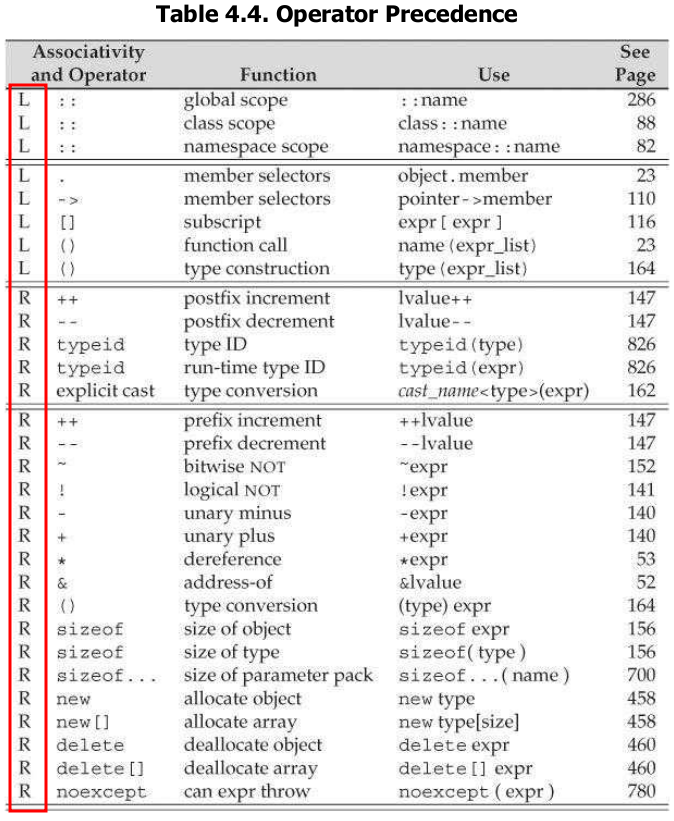
\includegraphics[height=0.7\textheight]{img/precedence.png}
    \end{figure}
\end{frame}

\begin{frame}{Short-circuit Evaluation}
    Logical operators \texttt{\&\&} and \texttt{||} are short-circuited:
    \begin{itemize}
        \item Both \texttt{\&\&} and \texttt{||} evaluates their left operand first.
        \item If the left operand of \texttt{\&\&} evalutes \blue{\texttt{false}}, the right operand will not be evaluated, and the whole expression evaluates \blue{\texttt{false}}.
        \item If the left operand of \texttt{||} evalutes \blue{\texttt{true}}, the right operand will not be evaluated, and the whole expression evaluates \blue{\texttt{true}}.
    \end{itemize}
\end{frame}

\section{In the End}

\begin{frame}{How Do We Learn C/C++?}
    The key is to learn to \blue{think in C/C++ way}!
    \pause
    \begin{itemize}
        \item Is it even possible for the compiler to do this?
        \pause
        \item What would happen if something is not like this?
    \end{itemize}
\end{frame}

\end{document}